\documentclass[b5paper,11pt]{article}
\bibliographystyle{plain}

\usepackage{geometry}
\usepackage{amssymb,amsthm,bm,mathrsfs,mathtools}
\usepackage[usenames]{xcolor}
\usepackage{hyperref}
\usepackage{graphicx,subcaption}
\graphicspath{{../"img/"}{../"figures/"}}

\usepackage{mycommands}
\newcommand{\numcircled}[1]{\raisebox{.5pt}{\textcircled{\raisebox{-.9pt} {#1}}}}
\newcommand{\Dmax}{\trdis_\mathsf{max}}
\newcommand{\InFmax}{\infid_\mathsf{max}}
\newcommand{\Psb}{\mathcal{P}_\mathrm{SB}}
\newcommand{\Odd}{\Omega_{\mathsf{DD}}}
\newcommand{\Opdd}{\Omega_{\mathsf{PDD}}}
\newcommand{\vOpdd}{\vec{\Omega}_{\mathsf{P}}}
\newcommand{\LO}[1]{\operatorname{LO}}
\newcommand{\alphat}{\widetilde{\alpha}}
\newcommand{\betat}{\widetilde{\beta}}

\newcommand{\Ppb}{\mathscr{P}_{\mathrm{0}}}
\newcommand{\Pcp}{\mathscr{P}_{\mathrm{c}}}
\newcommand{\wtP}{\widetilde{P}}
\newcommand{\wtH}{\widetilde{H}}
\newcommand{\wtO}{\widetilde{\Omega}}
\newcommand{\wtU}{\widetilde{U}}
\newcommand{\wt}[1]{\widetilde{#1}}

\newcommand{\HB}{H_\mathrm{B}}
\newcommand{\HSB}{H_\mathrm{SB}}

\newcommand{\Heff}{H_\mathrm{eff}}
\newcommand{\HeffB}{H_\mathrm{eff,B}}
\newcommand{\HeffSB}{H_\mathrm{eff,SB}}

\newcommand{\ep}{\Phi_\mathrm{SB}}
\newcommand{\wtep}{\widetilde{\Phi}_\mathrm{SB}}
\newcommand{\epB}{\Phi_\mathrm{B}}
\newcommand{\phiB}{\phi_\mathrm{B}}

\newcommand{\ctrl}{\mathrm{ctrl}}
\newcommand{\CDDn}{\mathrm{CDD}_n}
\newcommand{\rDD}{\mathrm{DD}}
\newcommand{\rmax}{\mathrm{max}}
\begin{document}
\section{Note on noisy gates}
Previously, we treated the DD control gates in an ideal manner, which implies instantaneous and noise-free pulses. In practice, of course, the control gates are neither instantaneous nor noise-free. Hence the analysis for ideal DD cannot be directly carried out.

The effects of quantum noise on the system can be generally modelled with CPTP channels, which need not be unitary. The introduction of non-unitarity is problematic as the error phase, which is used to study the efficacy of DD, can no longer be defined.
However, one may include some ancillary qubits to transform any quantum channel into a unitary evolution over the extended Hilbert space. For the analytical treatment below, we will always assume this dilation for the noisy gates. Hence, we can ascribe Hamiltonian generators for the noisy control gates. 
Such generator can be time-dependent and involves in the term necessary for the control in addition to various sources contributing to the noise. 
Focusing on the $i$th gate-interval,  we can write the total Hamiltonian:
\begin{equation}\label{eq:noisy-Hamiltonian}
 H(t) = H_e + H_c(t), \quad t_{i-1}< t \le t_i,
\end{equation}
where $H_e=H_\rB+H_\rSB$ is the error Hamiltonian between system and bath, $H_c(t)$ is the control Hamiltonian generating the gate $P_i$.
For the ideal case considered earlier, it is assumed $H_c(t) \propto \delta(t-t_i)$; then the corresponding time evolution operator is simply $P_i \upe^{-\upi \tau H_e} =P_i \upe^{-\upi \Omega}$. For the case of noisy gates, the control Hamiltonian $H_c(t)$ is not a delta spike and will only approximately generate the gate $P_i$.

In general, directly solving the DD time evolution operator $U(t_L,t_0)$ from $H(t)$ in \Eqref{eq:noisy-Hamiltonian} will not work, as the very large $H_c(t)$ integral in the matrix exponent will break the convergence condition for the Magnus series. Hence it is necessary to separate out the ``pure gate'' parts from the ``free evolution'' parts. We formally perform such separation  by  expressing the solution to unitary time evolution for the $i$th gate interval as:
\begin{equation}
 \wtU(t_i,t_{i-1})
 = P_i \upe^{-\upi \wtO_i}, 
\end{equation}
where the gate-dependent $\wtO_i$ replaces the free evolution generator $\Omega$ for ideal DD. 
We put tildes over operators to signify that the DD control gates are noisy. 
Similar to the ideal DD case, we can split the $P_i$s by defining $P_i=G_{i+1}^\dagger G_{i}$ and then,
\begin{equation}
\begin{aligned}
  \wtU_\rDD= \upe^{-\upi  G_L \wtO_L  G_L^\dagger} \ldots
  \upe^{-\upi G_2 \wtO_2  G_2^\dagger} \upe^{-\upi G_1\wtO_1G_1}\equiv\upe^{-\upi\wtO_\rDD} .
\end{aligned}
\end{equation}
Provided the noise being small, the $\wtO_i$s are small and we may use the Magnus formula to derive the leading order Magnus series as good approximation to $\wtO_\rDD$.
The overall goal is to figure out the conditions such that the noise-inflicted DD error phase $\wtep \equiv \norm{\wtO_{\rDD,\rSB}}$  is still reduced compared to the bare Hamiltonian error phase $\phi_\rSB = \norm{\Omega_{\rSB}}$. For simplicity, let us employ a single parameter $\eta$, which is defined later,  to quantify the noise strength associated with the gates.  The break-even condition is, in essence, to invert the inequality
\begin{equation}
 \wtep(\phi_\rB,\phi_\rSB,\eta) < \phi_\rSB,
\end{equation} 
and obtain an upper bound on the noise level $\eta<\eta_{\rmax}(\phi_\rB, \phi_\rSB)$.
To achieve this, we not only need an appropriate noise strength parameter $\eta$, but also correctly estimate the DD error phase function $\wtep(\phi_\rB,\phi_\rSB,\eta)$.  

 In the followings, we will mainly focus on the PDD to derive explicit break even conditions for various noise. But our analysis should be easily generalized to other DD sequences as well.







\subsection{Noisy pulses}
If the non-zero duration of $H_c(t)$ is much shorter than the gate interval,  the control gates can still be viewed as instantaneous pulses. In this section we consider noisy pulses, that is 
$H_c(t)\sim \delta(t-t_i)$, but does not produce the ideal gate.
The  time evolution operator for the $i$th gate interval becomes:
\begin{equation}\label{eq:npulses-Ui}
 \wtU(t_i,t_{i-1}) = \wtP_i \upe^{-\upi \Omega},
\end{equation}
where $\widetilde{P}_i$ is the noisy pulse version for the ideal $P_i$ gate and $\Omega=\tau H_e$ is the free evolution generator.
Let us also associate to $\wtP_i$ a Hermitian generator, which should be dominated by that of an ideal gate in addition to a small noise part:
\begin{equation}\label{eq:npulses-Pi}
 \widetilde{P}_i= \exp\left[ -\upi \left( \Omega_{P_i} +  \eta \Gamma_{P_i} \right)  \right],
\end{equation}
where $\Omega_{P_i}$ is responsible for the ideal gate $P_i = \exp(-\upi \Omega_{P_i})$ and supported only on the system; and $ \eta \Gamma_{P_i} $ is responsible for the noise and supported on the system-bath-ancilla composite in general. We have introduced the explicit small parameter $\eta$ to facilitate order tracking and normalized $\Gamma_{P_i}$. For PDD in particular, the sequence comprises only $X$ and $Z$ gates. 
And we may write the noisy $X$ and $Z$ pulses as:
\begin{equation}
\widetilde{X} = \upe^{-\upi ( \frac{\pi}{2} \sigma_1 + \eta\Gamma')},\quad
 \widetilde{Z} = \upe^{-\upi ( \frac{\pi}{2} \sigma_3 + \eta\Gamma'')},
\end{equation}
where $\Gamma'$ and $\Gamma''$ accounts for the noise in $\wt X$ and $\wt Z$.
We separate out the system part of these operators by $\Gamma' = \sum_i \sigma_i \otimes B'_i $ and $\Gamma''=\sum_i \sigma_i \otimes B''_i$, with $B'_i$ and $B''_i$ acting on the bath-ancilla product space. 
The time evolution for the noisy PDD sequence then becomes
\begin{equation}\label{eq:UPDD-gatedep}
 \begin{aligned}
\wtU_\rDD &=
 \widetilde{Z} \upe^{-\upi \Omega}
 \widetilde{X} \upe^{-\upi \Omega}
 \widetilde{Z} \upe^{-\upi \Omega}
 \widetilde{X} \upe^{-\upi \Omega}\\
 & = \upe^{-\upi  \Gamma_3} \upe^{- \upi\Omega_3}
 \upe^{-\upi  \Gamma_2}  \upe^{-\upi\Omega_2}
\upe^{-\upi  \Gamma_1} \upe^{-\upi\Omega_1}
\upe^{-\upi  \Gamma_0}  \upe^{-\upi \Omega_0},
\end{aligned}
\end{equation}
where $\Omega_i = \sigma_i \Omega \sigma_i$ as in the ideal case; and we define
$\upe^{-\upi  \Gamma_3}=\wt Z Z$, 
$\upe^{-\upi  \Gamma_2}=Z \wt X Y$,
$\upe^{-\upi  \Gamma_1}=Y \wt Z X$ and 
$\upe^{-\upi  \Gamma_0}=X \wt X$.
By keeping the first order in 
$\eta$, we can derive
\begin{equation}
 \begin{aligned}
  \Gamma_3 &= \eta(\sigma_0 \otimes B_0''- \frac{2}{\pi} \sigma_1 \otimes B_2'' 
  +\frac{2}{\pi}  \sigma_2 \otimes B_1'' + \sigma_3 \otimes B_3''),\\
  \Gamma_2 &= \eta(\sigma_0 \otimes B_0'- \sigma_1 \otimes B_1'
  +\frac{2}{\pi}  \sigma_2 \otimes B_3' + \frac{2}{\pi} \sigma_3 \otimes B_2'),\\
  \Gamma_1 &= \eta(\sigma_0 \otimes B_0''+ \frac{2}{\pi} \sigma_1 \otimes B_2'' 
  +\frac{2}{\pi}  \sigma_2 \otimes B_1'' - \sigma_3 \otimes B_3''),\\
  \Gamma_0 &= \eta(\sigma_0 \otimes B_0'+ \sigma_1 \otimes B_1'
  +\frac{2}{\pi}  \sigma_2 \otimes B_3' - \frac{2}{\pi} \sigma_3 \otimes B_2').
 \end{aligned}
\end{equation}
Every term on the exponent in \Eqref{eq:UPDD-gatedep}  is now at least linear in the smallness $\eta$ or $\norm{\Omega}$ and we can apply the Magnus formula to calculate $\widetilde\Omega_\mathrm{PDD}$. 
The first order Magnus term suggests:
\begin{equation}
 \wt\Omega_\rDD\up{1}= \sigma_0 \otimes (4B_0 + 2\eta( B'_0 + B''_0)) 
+ \sigma_2 \otimes \frac{4}{\pi}\eta(B_1''+B_3').
\end{equation}
The term that acts non-trivially on the system is proportional to $B_1''+B_3'$. 
Assuming no particular relation between the $X$ and $Z$ noise,  exact first order decoupling is lost. 
When the gate noise strength $\eta$ is at least of similar size as $\phi_\rSB$---the gate noise is typically stronger than the background noise in many experiments---the first order Magnus term would be of leading order in magnitude. And the error phase after PDD is reduced to a linear multiple in $\eta$. 
 we upper-bound the size of the first order coupling by:
\begin{equation}
 \wt\Phi_\rSB \approx \norm{ \frac{4\eta}{\pi}(B_1''+B_3')} \le \frac{8}{\pi}\eta.
\end{equation}
This results in the first order breakeven condition:
\begin{equation}
 \eta \le \frac{\pi}{8} \phi_\rSB.
\end{equation}
This condition indicates that in order to achieve noise suppression, the gate noise should be bounded by a fraction of the free evolution noise. If any observable improvement from DD is expected, the pulses must be very accurate in the first place.   On the other hand if $\eta\ll \phi_\rSB$, the existence of pulse noise contributes negligibly and the second oder term will be similar to the ideal PDD case. Hence to faithfully approximate the full $\wt\Omega_\rDD$, we may keep every term that is linear in $\eta$ and up to second order in the smallness $\phi_\rB$ or $\phi_\rSB$ (alternatively: second order in $\phi$). Focusing on the interaction part, the result becomes:
\begin{equation}
 \wt\Omega_{\rDD:\rSB} = \Omega_{\rDD:\rSB} +\sigma_2 \otimes \frac{4}{\pi}\eta(B_1''+B_3') + \cO(\eta\phi,\phi^3).
\end{equation}
Bounding the resulting error phase and applying triangular inequality, we have the second order breakeven condition:
\begin{equation}\label{eq:npulses-breakeven2}
   \eta \le \frac{\pi}{8} \phi_\rSB - \frac{\pi}{8}\Phi_\rSB^{(\mathrm{ub})}.
\end{equation}
We remark that this is a loose bound and tighter bound can be obtained by performing optimization on $\norm{\wt\Omega_{\rDD:\rSB}}$ akin to what we did for the ideal case, rather than using triangular inequality. But the current form is enough to serve our purpose. 
For verification, we numerically simulated PDD with noisy pulses and compare the results with our our break even conditions in \Figref{fig:pdd-noisy-pulse}. 
Specifically, for each fixed tuple of parameters $(\phi_\rB,\phi_\rSB,\eta)$, we randomly generate 300 sets of the Hermitian matrices $\{\Omega,\Gamma',\Gamma''\}$
satisfying the given parameters over a uniform distribution. Noisy PDD is simulated for each particular set of  bare Hamiltonian and noisy pulses; the noise reduction ratio $\wt\Phi_\rSB/\phi_\rSB$ is obtained and numerically maximized for the fixed $(\phi_\rB,\phi_\rSB,\eta)$. 
We used two figures to visualize the effect of noisy pulses. First is the deformation---or shrinking to be exact---of the noise removal region in the $(\phi_\rB,\phi_\rSB)$ phase diagram. Second is the dependence between the maximally allowed noise versus the free-evolution noise. From the figure we can see that our first order condition works well as long as the noise parameter $(\phi_\rB,\phi_\rSB)$ is weak and the second order condition is more universally applicable for a wider range of conditions.



 \begin{figure}
 \centering
 \begin{subfigure}{0.45\linewidth}
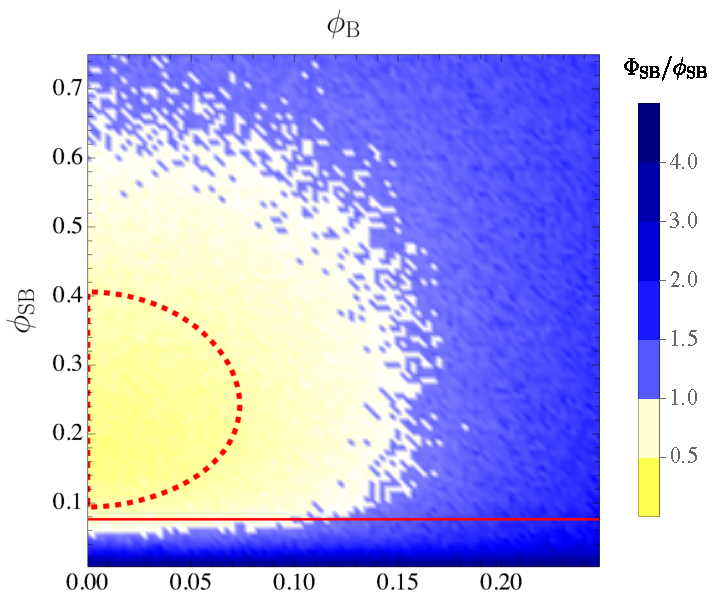
\includegraphics[height=0.8\linewidth]{pdd-noisypulse1}
\caption{$\eta =0.03$.}
\label{fig:pdd-noisy-pulse1}
\end{subfigure}
\hfill
\begin{subfigure}{0.45\linewidth}
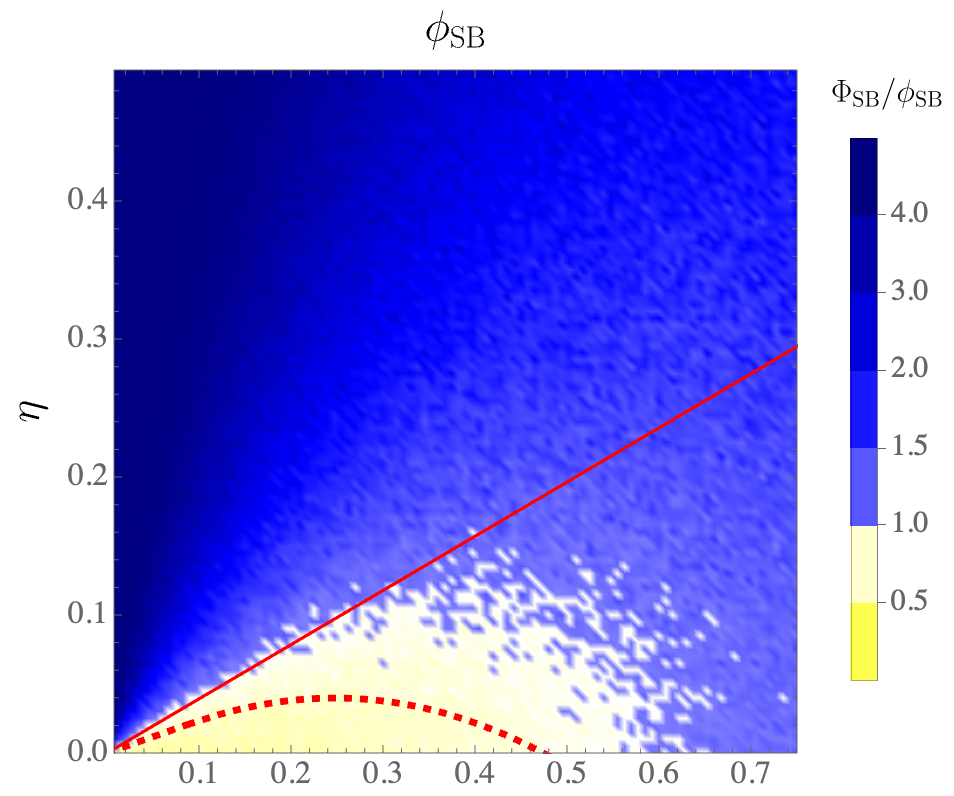
\includegraphics[height=0.8\linewidth]{pdd-noisypulse2}
\caption{$\phi_\rB =0.05$.}
\label{fig:pdd-noisy-pulse2}
\end{subfigure}
\caption{The maximal noise reduction ratio for the noisy PDD. A point is colored yellow if the noise is reduced after PDD.  The first order condition is indicated with the red solid line while the second order condition is indicated with the red dashed line. }
\label{fig:pdd-noisy-pulse}
\end{figure}



We now examine the special scenario where the first order decoupling is exact, which requires $B''_1+B'_3=0$. It can be shown that this condition actually corresponds to a ``weakly gate-dependent'' noise model:
\begin{equation}\label{eq:gateindep1}
 \wtP_i = P_i \upe^{-\upi \eta \Gamma + \cO(\eta^2)},\ \forall i.
\end{equation}
For the most generic noisy pulses, we can write introduce the gate-noise decomposition $\wtP_i = P_i \upe^{-\upi \eta \Gamma_i}$. The weak gate-dependence assumption is demanding that the variance in $\Gamma_i$  
is at most on the order of the smallness parameter $\eta$.
 That is, the dependence of the noise on the gate is weak. If this condition is 
 satisfied, then the time evolution readily reduces to the ideal DD case by replacing $\Omega=\tau H$ for free evolution with an effective Hamiltonian $\wtO$ such that
\begin{equation}
\upe^{-\upi \wtO}=\upe^{-\upi \eta \Gamma}\upe^{-\upi \Omega}.
\end{equation}
Since $\Gamma$ and $\Omega$ are both small, as required for DD to work,
one may invoke the BCH formula to get $\wtO$ as a series of nested commutators. 
The already established map $\Omega\to \Omega_{\rDD}$ for the idea-pulse DD sequence can then be reused to estimate $\Omega_{\rDD}$
Naturally, we recover exact first order decoupling for PDD. To derive the break-even condition for such weakly gate-dependent noise, 
we retain the BCH series to the second order term, and then apply triangular inequality to derive the upper bounds for $(\widetilde\phi_\rB,\widetilde{\phi}_\rSB) \equiv( \norm{\wtO_\rB}, \norm{\wtO_\rSB})$:
\begin{equation}\label{eq:comb-bound}
\left\{
\begin{aligned}
 \widetilde\phi_\rB &\lesssim (\eta + \phi_\rB)(1+\eta + \phi_\rSB) \equiv \widetilde\phi_\rB^{(\mathrm{ub})}\\
 \widetilde\phi_\rSB &\lesssim (\eta + \phi_\rSB) (1+\eta + \phi_\rB)\equiv \widetilde\phi_\rSB^{(\mathrm{ub})}
\end{aligned}
\right..
\end{equation}
With this, we can bound the error phase relevant for this noisy-pulse situation under the different schemes by replacing $\phi_\rB$ and $\phi_\rSB$ for the ideal case with their noisy upper bounds: 
\begin{equation}
 \widetilde\Phi_\rSB \le \Phi_\rSB(\widetilde\phi_\rB^{(\mathrm{ub})}  ,\widetilde\phi_\rSB^{(\mathrm{ub})} ) < \phi_\rSB.
\end{equation}
Further bounding the right hand side by $\phi_\rSB$ then gives us the condition for the break-even points.

The above analysis is generic and applies to all DD schemes with gate-independent noise. 
The resulting bound is general, but could be suboptimal for a specific DD scheme and a specific type of pulse imperfection. Below, we examine a concrete examples of imperfections  for PDD: 
global unitary error in the control gates,  which results in the noisy pulse 
\begin{equation}
\widetilde P_i=P_i\upe^{-\upi \bm{\theta}\cdot\bm\sigma},\ \forall i.
\end{equation}
We use the notation $\bm\sigma=(\sigma_1,\sigma_2,\sigma_3)$, and $\bm\theta\equiv (\theta_1,\theta_2,\theta_3)$ with $\theta_i$ real constants---taken as small for weak noise---that parameterize the unitary error.  This can arise from, for example, a systematic calibration error in the pulse control leading to a consistent over or under rotation. In this situation, $\Gamma\equiv \bm\theta\cdot\bm\sigma$ acts only on the system and does not have a pure bath term. In the appendix, we derive an tighter bound:
\begin{equation}\label{eq:eff-Hami-tcp}
\left\{
\begin{aligned}
\widetilde{\phi}_\rB &\le \phi_\rB + \frac{1}{3}\theta  \phi^2_\rSB  \\
\widetilde{\phi}_\rSB &\le \phi_\rSB +  \theta^2  \phi_\rSB  \\
\end{aligned}    \right.,
\end{equation}
where $\theta \equiv \norm{\bm \theta}$ is the rotation angle associated with the gate error.
Assuming the noise to be small, we may only use the leading order 
approximation, which is by itself accurate to the second order. 
Substituting the upper bounds to  $\Phi_\rSB(\wt\phi_\rB,\wt\phi_\rSB)$ and keeping the leading order terms,  we can predict the following simplified bound for PDD:
\begin{equation}\label{eq:npdd-bound-simple}
2\phi_\rB^2 + \frac{(\theta+\phi_\rSB)^4}{4\phi_\rSB^2}\le \frac{1}{16},
\end{equation}
From this inequality, the globally maximally allowed $\theta$ can be found at $\phi_\rB=0$, $\phi_\rSB=1/8$ with
$\theta_\mathrm{max}= 1/8$. Furthermore, we can solve for $\theta$ in terms of $\phi_\rB$ and $\phi_\rSB$ to arrive at the noise threshold for the rotation angle:
\begin{equation}\label{eq:npdd-err-thres}
    \theta \le (1-32\phi_\rB ^2)^{\frac{1}{4}} \sqrt{\frac{\phi_\rSB}{2} }-\phi_\rSB
    \quad \lesssim \sqrt{\frac{\phi_\rSB}{2}}.
\end{equation}
It states that for the regime where the the free evolution noise is small, gate noise should at most be on the order of the square root of the free evolution noise. This  is quite different from the generic noise case where the upper bound dependence in $\phi_\rSB$ is linear. 


\subsection{Gates of finite duration}
In reality the control Hamiltonian cannot be made infinitely large and 
has a finite duration. This contributes to an extra source of noise in addition
to the free evolution noise.  In this section, we consider such type of noise. 

The simplest example is that of the finite width rectangular pulses. Assuming the gate pulse is $\tau_p$, the Hamiltonian  for the $i$th gate interval is split into two constant pieces: $H=H_c+H_e$ for $t_i -\tau_p  < t \le t_{i}$ when the control is in applied, while $H=H_e$ for other times. The control Hamiltonian is assumed to satisfy $P_i = \upe^{-\upi \tau_p H_c }$.
A similar noise model was first considered in the original CDD paper~\!\cite{khodjasteh2007performance} for the convergence proof. Let us work out a slightly more involved model where apart from the finite width, the control Hamiltonian is also infested with a small control error denoted by $\epsilon\Gamma_i$, with $\max{(\Gamma_i)}=1, \forall i$ and $\epsilon\ll 1$.  Namely, without the environment noise, the $i$th control gate
is $ \upe^{-\upi (\Omega_{P_i} +\epsilon \Gamma_i)}$, where $\upe^{-\upi \Omega_{P_i} }$ is the ideal gate. 
We write solution to the time-evolution operator as:
\begin{equation}
 \wt U(t_{i},t_{i-1}) =  \upe^{-\upi (\Omega_{P_i} +\epsilon \Gamma_i+
 (\tau_p/\tau) \Omega)}  \upe^{-\upi (1-(\tau_p/\tau)) \Omega}.
\end{equation}
The ratio $\tau_p/\tau$ between the pulse width and the gate interval and is typically considered to be small, hence so is the noise term $(\tau_p/\tau)\Omega$. Despite having a finite gate width,  one can immediately convert such case to the instantaneous pulse model.
To do so, one simply need to replace the free evolution generator with $ (1-(\tau_p/\tau)) \Omega$ and the pulse noise generator  with $\epsilon \Gamma_i + (\tau_p/\tau) \Omega$ in \Eqref{eq:npulses-Pi}.
In terms of PDD with noisy pulses considered previously, to obtain the Magnus series for the finite width scenario, all we need is to make the substitutions $B_i \to (1-(\tau_p/\tau)) B_i$, $\eta B_i' \to (\tau_p/\tau) B_i + \epsilon B_i'$ and $\eta B_i'' \to (\tau_p/\tau) B_i + \epsilon B_i''$ in the original results. Using the first order expansion, we estimate the error phase as 
\begin{equation}
\norm{ \wt\Omega_{\rDD:\rSB}\up{1} }\le \frac{4\sqrt{2}}{\pi} (\frac{\tau_p}{\tau})\phi_\rSB +  \frac{8}{\pi} \epsilon.
\end{equation}
We see that the error phase contribution from the finite width is automatically on the second order smallness if we assume $\tau_p\ll \tau$, this is different from the control error, which contributes to the first order smallness. 
This suggests DD is very tolerant to the finite width error. If the gate control error is absent, the first order breakeven condition suggests
\begin{equation}
 \tau_p/\tau \le \frac{\pi}{4\sqrt{2}}\approx 0.555,
\end{equation}
to be sufficient for noise reduction.
For the second order breakeven condition, we can simply substitute the effective noise strength $\eta = \epsilon + \frac{\tau_p}{\tau}\phi_\rSB$ to \Eqref{eq:npulses-breakeven2}.

Let us for now assume that without the system-bath coupling, the control Hamiltonian $H_c(t)$ will generate the exact control gate $P_i$ over the $i$th gate interval. This condition can be written as
\begin{equation}
 P_i = \cT_{\leftarrow} \exp{\left[-\upi \int_{t_{i-1}}^{t_i} H_c(t) dt\right]},
\end{equation}
where $\cT_{\leftarrow} $ is the Dyson series time-ordering operator. 
 
For the noisy gates, 
we have the time-evolution operator
\begin{equation}
 \wtP_{\sigma_\alpha} =\exp\left[{-\upi \left(\frac{\pi}{2}\sigma_\alpha + \frac{1}{2}\bm \theta_\alpha\cdot \bm \sigma
 + r \Omega
 \right)}\right],  \ \alpha=1,3.
\end{equation}



 In this section, we assume that the noise is 
\begin{equation}\label{eq:Pi_approx}
 P_i \approx\cT_{\leftarrow} \upe^{-\upi \int_{t_{i-1}}^{t_i} H_c(t) \dd t }.
\end{equation}


\bibliography{references}
\end{document}